


\newcommand{\resultsfigwidth}{1.14in}
\renewcommand{\resultscropwidth}{0.69in}

\newcommand{\cropship}[1]{
  \makecell{
%   \includegraphics[trim={350px 450px 350px 250px}, clip, width=\resultscropwidth]{#1} \\
%   \includegraphics[trim={200px 400px 500px 300px}, clip, width=\resultscropwidth]{#1}
  \includegraphics[trim={331px 438px 325px 218px}, clip, width=\resultscropwidth]{#1} \\
  \includegraphics[trim={352px 298px 320px 374px}, clip, width=\resultscropwidth]{#1}
  }
}


\newcommand{\croplego}[1]{
  \makecell{
%   \includegraphics[trim={270px 300px 430px 400px}, clip, width=\resultscropwidth]{#1} \\
%   \includegraphics[trim={450px 460px 250px 240px}, clip, width=\resultscropwidth]{#1}
  \includegraphics[trim={440px 420px 218px 238px}, clip, width=\resultscropwidth]{#1} \\
  \includegraphics[trim={541px 289px 91px 343px}, clip, width=\resultscropwidth]{#1}
  }
}

\newcommand{\cropmic}[1]{
  \makecell{
  % left bottom right top
%   \includegraphics[trim={200px 580px 500px 120px}, clip, width=\resultscropwidth]{#1} \\
%   \includegraphics[trim={400px 350px 300px 350px}, clip, width=\resultscropwidth]{#1}
  \includegraphics[trim={352px 261px 274px 365px}, clip, width=\resultscropwidth]{#1} \\
  \includegraphics[trim={182px 583px 504px 103px}, clip, width=\resultscropwidth]{#1}
  }
}

\newcommand{\cropmat}[1]{
  \makecell{
  % left bottom right top
%   \includegraphics[trim={200px 580px 500px 120px}, clip, width=\resultscropwidth]{#1} \\
%   \includegraphics[trim={400px 350px 300px 350px}, clip, width=\resultscropwidth]{#1}
  \includegraphics[trim={194px 274px 402px 322px}, clip, width=\resultscropwidth]{#1} \\
  \includegraphics[trim={418px 363px 258px 313px}, clip, width=\resultscropwidth]{#1}
  }
}

% \afterpage{\clearpage}
\begin{figure}[t]
\centering
\scriptsize
\begin{tabular}{@{}c@{}c@{}c@{}c@{}c@{}c@{}}
\makecell[c]{
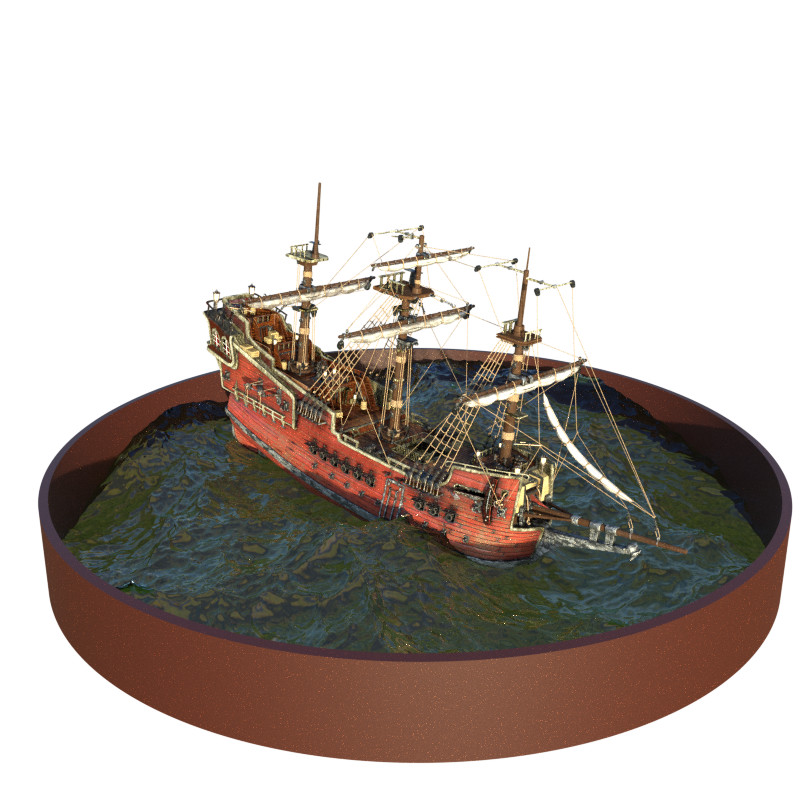
\includegraphics[trim={0px 0px 0px 100px}, clip, width=\resultsfigwidth]{figs/synth_results/ship/gt.jpg}
\\
\scenename{Ship}
}
&
\cropship{figs/synth_results/ship/gt.jpg} &
\cropship{figs/synth_results/ship/nerf.jpg} &
\cropship{figs/synth_results/ship/llff.jpg} &
\cropship{figs/synth_results/ship/srn.jpg} &
\cropship{figs/synth_results/ship/nv.jpg} \\
\makecell[c]{
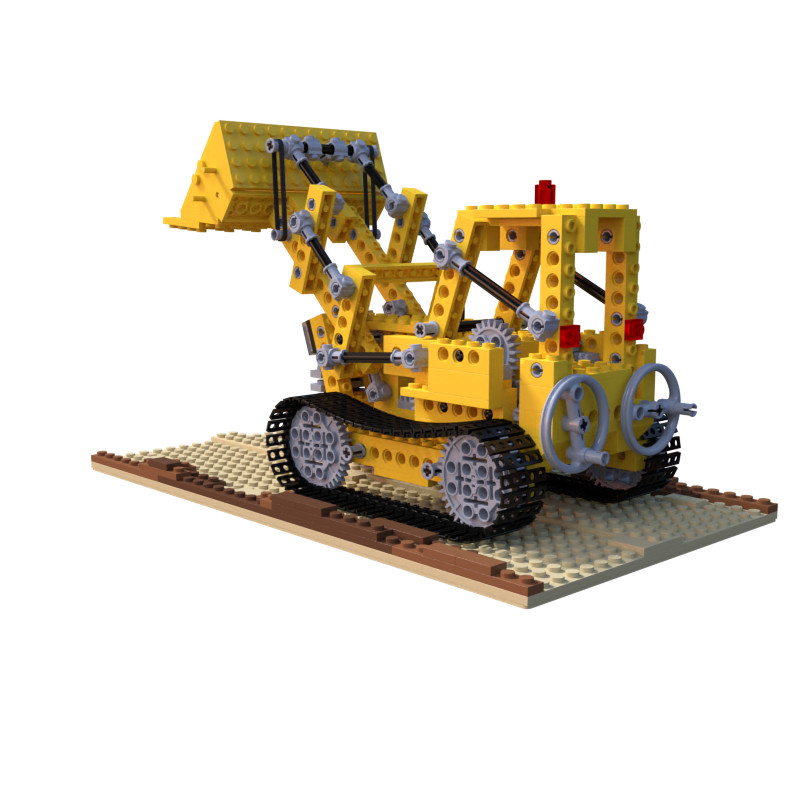
\includegraphics[trim={86px 178px 18px 100px}, clip, width=\resultsfigwidth]{figs/synth_results/lego/gt.jpg}
\\
\scenename{Lego}
}
&
\croplego{figs/synth_results/lego/gt.jpg} &
\croplego{figs/synth_results/lego/nerf.jpg} &
\croplego{figs/synth_results/lego/llff.jpg} &
\croplego{figs/synth_results/lego/srn.jpg} &
\croplego{figs/synth_results/lego/nv.jpg} \\
\makecell[c]{
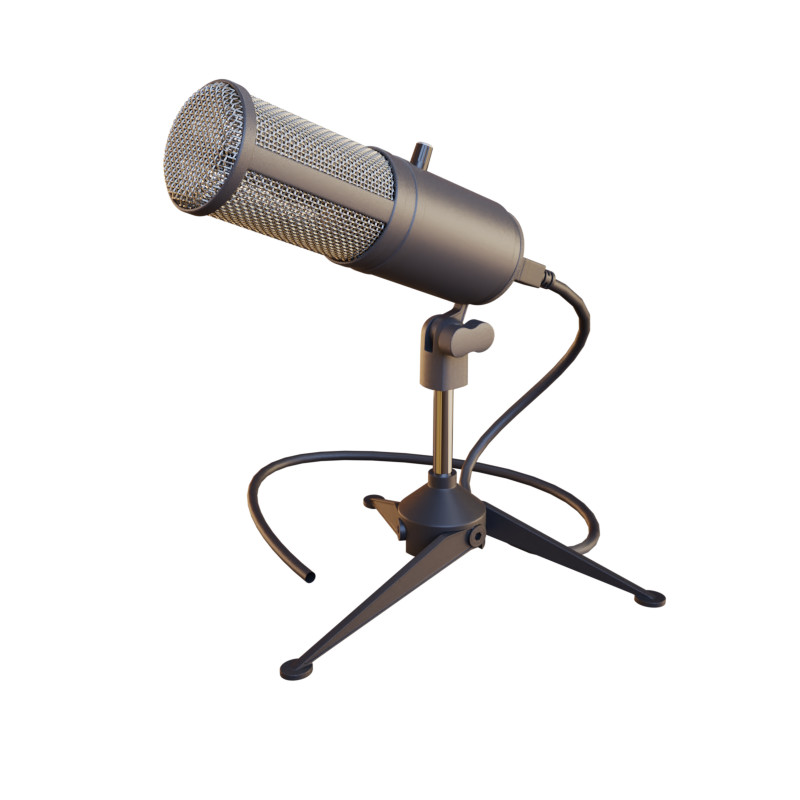
\includegraphics[trim={95px 95px 65px 50px}, clip, width=\resultsfigwidth]{figs/synth_results/mic/gt.jpg} 
\\
\scenename{Microphone}
}
&
\cropmic{figs/synth_results/mic/gt.jpg} &
\cropmic{figs/synth_results/mic/nerf.jpg} &
\cropmic{figs/synth_results/mic/llff.jpg} &
\cropmic{figs/synth_results/mic/srn.jpg} &
\cropmic{figs/synth_results/mic/nv.jpg} \\
\makecell[c]{
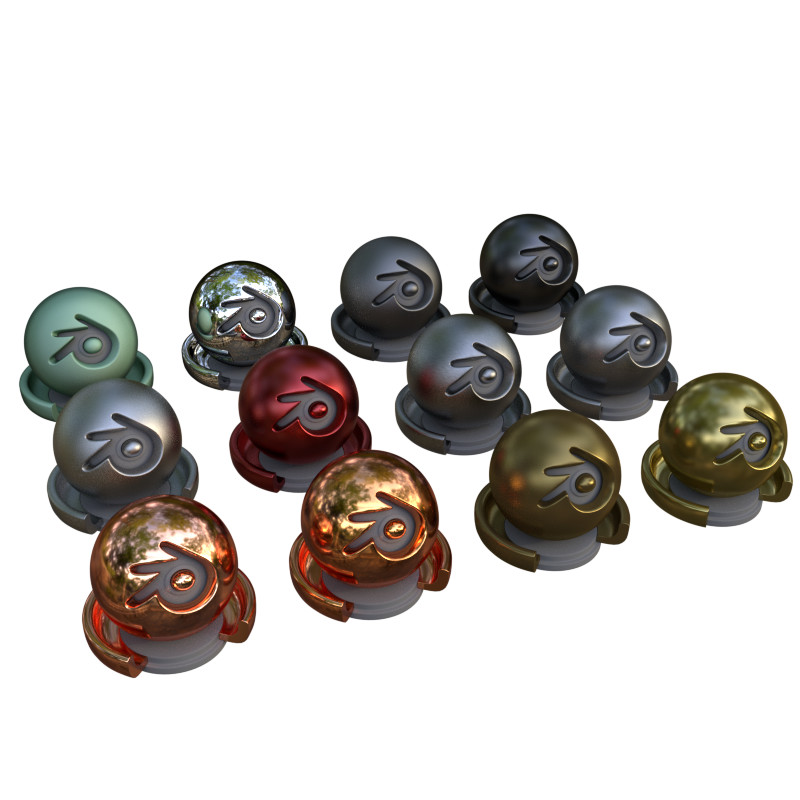
\includegraphics[trim={0px 0px 0px 0px}, clip, width=\resultsfigwidth]{figs/synth_results/materials/gt.jpg} 
\\
\scenename{Materials}
}
&
\cropmat{figs/synth_results/materials/gt.jpg} &
\cropmat{figs/synth_results/materials/nerf.jpg} &
\cropmat{figs/synth_results/materials/llff.jpg} &
\cropmat{figs/synth_results/materials/srn.jpg} &
\cropmat{figs/synth_results/materials/nv.jpg} \\
& Ground Truth & NeRF (ours) & LLFF~\cite{mildenhall19} & SRN~\cite{srn} & NV~\cite{neuralvolumes}
% \multicolumn{2}{c}{Ground Truth} & Our Model & LLFF~\cite{mildenhall19} & SRN~\cite{srn} & NV~\cite{neuralvolumes}
\end{tabular} 
\caption{Comparisons on test-set views for scenes from our new synthetic dataset generated with a physically-based renderer. Our method is able to recover fine details in both geometry and appearance, such as \scenename{Ship}'s rigging, \scenename{Lego}'s gear and treads, \scenename{Microphone}'s shiny stand and mesh grille, and \scenename{Material}'s non-Lambertian reflectance. LLFF exhibits banding artifacts on the \scenename{Microphone} stand and \scenename{Material}'s object edges and ghosting artifacts in \scenename{Ship}'s mast and inside the \scenename{Lego} object. SRN produces blurry and distorted renderings in every case. Neural Volumes cannot capture the details on the \scenename{Microphone}'s grille or \scenename{Lego}'s gears, and it completely fails to recover the geometry of \scenename{Ship}'s rigging.}
% \caption{Comparisons on test-set views for $360^\circ$ scenes from our new synthetic dataset generated with a physically-based renderer. Our method is able to recover high-frequency details in both geometry and appearance, such as the rigging on \scenename{Ship}, the gear and treads in \scenename{Lego}, and the shiny stand and mesh grille in \scenename{Microphone}. LLFF struggles to compute accurate depths on this data because the baseline between inputs is large, resulting in banding artifacts on the \scenename{Microphone} stand and warped patches of scene content inside and underneath the \scenename{Lego} object. SRN does not have the representational power to represent complex geometry or appearance, and it produces blurry and distorted renderings in every example. Neural Volumes produces reasonable geometry in most cases but cannot capture the high-frequency details on the \scenename{Microphone} grille or \scenename{Lego} gears and bricks, and it completely fails to recover the fine geometry of the rigging on \scenename{Ship}.}
% \caption{Comparisons on test-set views for scenes from our new synthetic dataset. LLFF struggles to compute accurate depths on this data because the baseline between inputs is large, resulting in tearing and ghosting artifacts. SRN does not have the representational power to represent complex geometry or appearance. }
% \caption{Comparisons on test-set views for scenes from our new synthetic dataset. LLFF struggles to compute accurate depths on this data because the baseline between inputs is large, resulting in tearing and ghosting artifacts. SRN does not have the representational power to represent complex geometry or appearance. Neural Volumes is hampered by an underlying $128^3$ resolution voxel grid representing the scene. By comparison, our method excels at representing fine details even in highly complex scenes.}
\label{fig:synthresults}
\end{figure}